%!TEX root = thesis.tex
\chapter{Bibilography Review} \label{chap:sota}

\section*{}

% Neste capítulo é descrito o estado da arte e são apresentados trabalhos
% relacionados para mostrar o que existe no mesmo domínio e quais os problemas
% em aberto. Deve deixar claro que existe uma oportunidade de desenvolvimento
% que cobre alguma falha concreta .

% O capítulo deve também efetuar uma revisão tecnológica às principais
% ferramentas utilizáveis no âmbito do projeto, justificando futuras escolhas.

This chapter presents a summary and analysis of some works related to the use of Repast and JADE frameworks in the development of MAS. The related
work is sorted in four categories.

The first category includes a discussion about existing works on integrating both JADE and Repast simultaneously by developing a middleware framework.  While the goal of this thesis is not to use both frameworks simultaneously, these works give a valuable insight into the shortcomings of both frameworks as well as providing some interesting comparisons between their features. The second category includes discussion about implementations of these protocols in Repast. Then, the third category presents some existing Java code generation and transformation tools. These tools will give support to the automation of code refactoring, detection of code patterns and library calls. This chapter ends with a summary of the bibliography review and an overview of the most interesting topics approached in this chapter.

\section{JADE and Repast integration}
JADE is a very popular framework for developing MAS, providing an infrastructure that allows the programmer to create a distributed system in a very transparent way. As discussed before, in the motivation for this thesis, JADE is not the best tool to develop a MABS, not only because it lacks the visualization tools that other frameworks provide for displaying data about agent behavior, but also because due to its multi threaded architecture JADE has performance issues when the system comprises a large number of agents. Following are two frameworks created to bridge these two worlds of MAS development and simulation by integrating Repast and JADE in the same platform by means of a middleware.

\subsection{MISIA: Middleware Infrastructure to Simulate Intelligent Agents}

	MISIA is a middleware whose goal is to enhance the simulation of intelligent agents and to allow the visualization and analysis of agent's behavior. Not only does MISIA allow ``simulation, visualization and analysis of the agent’s behavior'', but also ``makes use of technologies for the development of multi-agent systems known and widely used, and combines them so that it is possible to use their capabilities to build highly complex and dynamic systems.'' In Garcia \textit{et al}, the authors chose to develop this framework on top of JADE and Repast Symphony. Their reasoning lies on the widespread use of JADE as an agent-based software development middleware, on Repast being simple and well documented and finally on both frameworks being open source. \cite{garcia2011misia}


	Most platforms like JADE lack organizational features and support for simulation constraints - this infrastructure must be developed by the programmer. The main concept introduced to JADE by MISIA is the concept of time - synchronization is fundamental for simulation. MISIA also brings the possibility to develop open MAS in Repast by taking advantage of JADE implementation of FIPA protocols.

	\begin{figure}[h]
	  \begin{center}
	    \leavevmode
	    \includegraphics[width=.7\textwidth]{misia}
	    \caption{Functional structure of MISIA \cite{garcia2011misia}}
	    \label{fig:misiadiagram}
	  \end{center}
	\end{figure}

	As illustrated in the diagram on figure \ref{fig:misiadiagram}, MISIA consists of three layers of components: a layer of contact with Repast; an intermediate layer between the two frameworks; a layer that interfaces with JADE and enables the concept of time in that framework.

	The purpose of the `JADE layer' is for JADE's agents to perform their actions in each tick - the smallest unit of time in a Repast-based simulation. The synchronization of JADE's agents is made by informing them about the current tick. MISIA uses an agent for this - dubbed `synchronizer' - that acts as a notifier. Furthermore, FIPA protocols are implemented with a wrapper that adapts them to Repast ticks.

	Besides creating a wrapper on JADE's agents and FIPA protocols, an extra agent was included in the Repast layer. This means that for each agent created with MISIA, there are actually two agents being created. This layer also lets the synchronizer know that a new tick has passed.

\subsection{JREP - Extending Repast Symphony for JADE Agent Behavior Components}
	In Gömer \textit{et al} \cite{gormer2011jrep}, the authors propose JREP, another platform for integrating JADE and Repast Symphony in the same framework, by means of a middleware. To demonstrate its use, the authors present an example of a smart airport and how it can be simulated using JREP.

\begin{quote}
	``JREP [is] a novel integration of JADE and Repast Symphony that efficiently combines the macro and micro perspective with an interaction layer. It allows to see not only the overall system behavior, but also the individual together with its interests, goals and the communication to
	others for local coordination and cooperation. Scheduling of the agents, (time) synchronization and the registration of new agents with the environment has been solved.'' \cite{gormer2011jrep}
\end{quote}

	The rationale for their choosing of JADE and Repast Symphony as working platforms is well defined:
	Repast provides statistical functions, real-time monitoring, graphs and history recording; it also supports external statistical programs and has good execution speed.
	JADE, on the other hand, is pointed as having a highly efficient message transport layer. 

	JREP's architecture is similar to that of MISIA. There are three layers where the first one, called \textit{macro level} interacts with Repast, providing the scheduling mechanism; the second one, which they called \textit{micro level}, interacts with JADE and contains the behavior objects and the third one, called \textit{interaction level} which handles agent interaction using FIPA ACL.
	Agents in JREP are represented as both a Repast Agent and a JADE Agent. The main difference to MISIA is that in JREP the Repast Agent contains the reference to the respective JADE agent while is MISIA this was handled by an intermediate layer.

\subsection{Similar work}
	Other works related to integration of features from Repast and JADE are available. This, however, is not the main focus of this thesis since its goal is not to use both frameworks simultaneously. That said, there is some interest in these works, as I explained in the beginning of this chapter. 

% end % JADE and Repast integration

\section{FIPA standards in Repast}
	MISIA and JREP both attempted to complement Repast's lack of communication protocols by creating an interface with JADE's implementation of FIPA interaction protocols. 

	Open source projects exist that contemplate the use of FIPA ACL as a library, but none was found to be actively maintained or properly documented. Therefore, this thesis will contemplate the creation of a Java library that brings FIPA standards to Repast.
% end % FIPA standards in Repast


\section{Code generation}
	There are multiple ways to tackle the problem of code transformations, as described in this thesis. The brute force approach would be to parse the source code, create an abstract syntax tree (AST), which represents all code constructions in a program, perform certain transformations in the tree, and then generate back the code from the new AST. Fortunately, there are free and open source projects that developers can use to do exactly this with significantly reduced effort. From the available tools, I selected the ones that are the most relevant to this thesis, i.e. tools for Java code transformation that are open source, well documented and still supported. 

\subsection{Eclipse Java Development Tools (JDT)}

	The Java Development Tools are are a group of plug-ins that provide Eclipse the necessary means to become a full-featured Java IDE.
	These tools make up what we perceive as the ``Eclipse IDE'' and programmers can use these libraries in their Java projects and perform tasks that require a certain introspection of the code itself. Some of the possibilities presented by Eclipse JDT that could be interesting for this thesis are the creation of projects (in runtime and programmatically) which would allow the generated code to be shown immediately in the IDE; accessing projects in the workspace, allowing the programmer to access the project's code; finding calls to methods, very useful for mapping library calls from one framework to the other (for instance) and AST parsing, for a lower level parsing of code, allowing to directly manipulate methods and data structures \cite{eclipseJDT}.

	JDT can be broken down into five main components: 

	\begin{description}
		\item[APT] - Annotation Processing Tool\hfill \\
  			This component can be used to parse annotations in the code. Annotations are a Java construction introduced in Java 5 and can be used to add meta information about classes, objects and methods. These annotations can then be parsed by frameworks that use the POJO (plain old Java objects) that enclose them. As an example in the context of the code generation tool, annotations could be used to select entities like agents or data structures in a JADE project that would then be visualized in a Repast chart.
		\item[Core] - Java IDE headless infrastructure \hfill \\
  			The core for the Java IDE, it allows to transverse the Java element tree and find package fragments, compilation units, binary classes, types, methods and fields. This tool could be useful for mapping methods and library calls from one framework to another.
		\item[Debug] - Debug support for Java\hfill \\
  			This tool makes the debug facilities of Eclipse possible. It provides functionalities such as execution control and contextual expression evaluation. It will probably not be very useful in the context of this thesis
		\item[Text and UI] - Java editing support and Java IDE user interface \hfill \\
  			These components make development in Eclipse possible by providing a GUI for code editing, enriched with syntactic errors highlighting, among other interesting aids. This component is not immediately necessary for the development of the code generation tool.
	\end{description}


\subsection{Spoon - Program Analysis and Transformation in Java}
	Spoon is a tool created to take advantage of the new features introduced on the release of Java 5, namely annotations and generics. It is a Java transformation tool that uses annotation processing, compile-time reflection and templates in a pure-Java environment to enable programmers to create their own platforms for code transformations. As illustrated by figure \ref{fig:spoon-compile}, these transformations occur on compile time and annotations are used as parameters for compilation. The programmer uses plain Java code to define the transformations that should occur, for instance, adding code snippets to the beginning of a method in a class. Finally, Spoon can be seamlessly integrated in an IDE such as Eclipse \cite{spoon,pawlak2006spoon}.

	\begin{figure}[h]
	  \begin{center}
	    \leavevmode
	    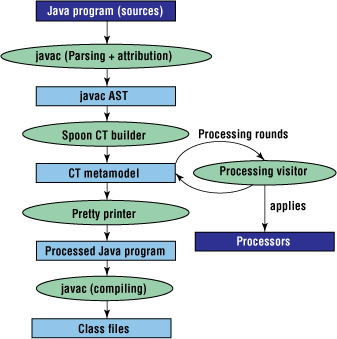
\includegraphics[width=.5\textwidth]{spoon-compile}
	    \caption{Spoon compile-time processing \cite{pawlak2006spoon}}
	    \label{fig:spoon-compile}
	  \end{center}
	\end{figure}

\subsection{ATL - ATL Transformation Language }
	ATL - \emph{ATLAS Transformation Language}, is both the name of a language and its enclosing plug-in and allows the creation of model transformations. Unlike JDT and Spoon analyzed before, ATL does not focus on applying transformations to the source code.

	\begin{figure}[h]
	  \begin{center}
	    \leavevmode
	    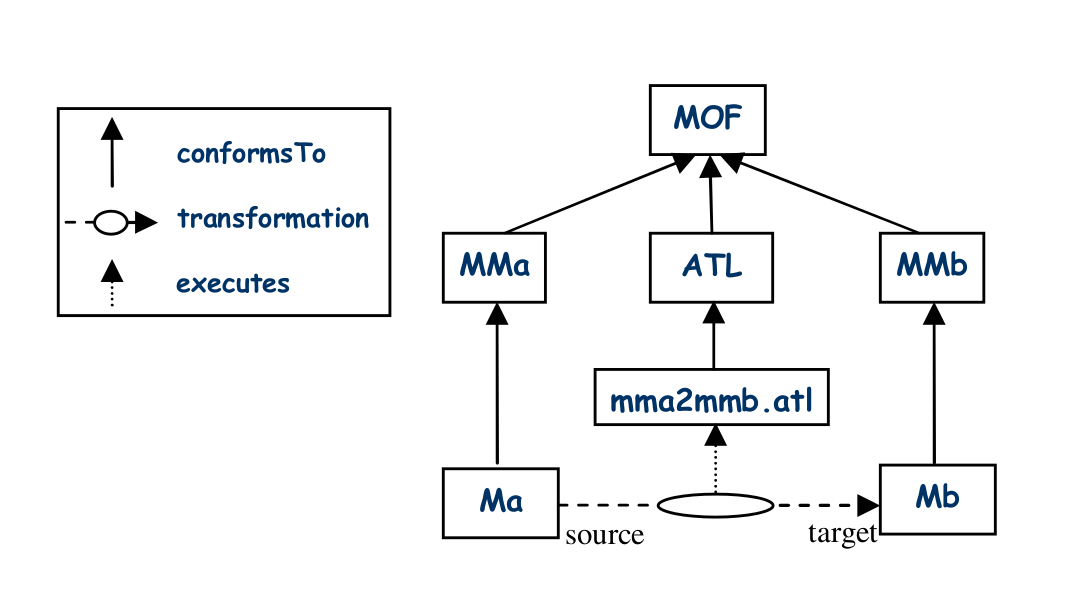
\includegraphics[width=.7\textwidth]{atl}
	    \caption{Overview of ATL transformational approach \cite{jouault2006transforming}}
	    \label{fig:so-atl-wow}
	  \end{center}
	\end{figure}

	\begin{quote}
		``ATL is applied in a transformational pattern shown in Fig. 1 . In this pattern a source model Ma is transformed into a target model Mb according to a transformation definition mma2mmb.atl written in the ATL language. The transformation definition is a model. The source and target models and the transformation definition conform to their metamodels MMa, MMb, and ATL respectively. The metamodels conform to the MOF metametamodel.''
	\end{quote}

	As explained in Jouault \emph{et al} and as illustrated in figure \ref{fig:so-atl-wow} by the same authors, ``a source model Ma is transformed into a target model Mb according to a transformation definition mma2mmb.atl written in the ATL language'', which is also a model itself. The three must conform to their respective metamodels MMa, MMb and ATL which then conform to the metametamodel MOF.
% end % Code generation tools


\section{Summary}
Although the specific problem of converting code between JADE and Repast has not been approach before in the available literature, it is clear that some related work is useful in the definition of a solution proposed in this thesis. JREP and MISIA show is that interoperability between the two frameworks is possible and helped defining the limitations of each framework. The usefulness of these works is limited, though, since the source code is not readily available and it is unknown if either project is still being developed and supported. Also, one of the goals proposed in the Introduction refers to the ability to generate code with introducing extensive changes to the original code. What JREP and MISIA propose is a platform to build new systems from the beggining using JADE and Repast.

Further testing is necessary to determine which of the code generation approaches proposed by the tools reviewed in this report should be used. As shown above, these tools provide interesting features and different methodologies to developers who wish to apply transformations on the source code of their projects in an automated way. An integration of these tools could prove to be the best approach, allowing the creation of an Eclipse plug-in with JDT and simplifying code transformations using simple Java constructions with Spoon or the specific transformation language of ATL.

\begin{table}[h]
	\caption{Comparison of code generation tools}
	\label{tab:codetools}
	\begin{center}
		\begin{tabular}{l|ccc}
		\hline

		\hline
		\textbf{} & \textbf{ATL} & \textbf{Spoon} & \textbf{JDT} \\
		\hline
			Language & ATL 		& Java 		& Java \\
		\hline
			License & EPL 		& CeCILL-C 	& EPL \\
					& (FOSS) 	& (FOSS)	& (FOSS) \\
		\hline
			Annotation Processing & No & Yes & Yes \\
		\hline
			AST parsing & No & Yes & Yes \\
		\hline
		\end{tabular}
	\end{center}
\end{table}

Table \ref{tab:codetools} presents a summary of the comparison of these three tools in an attempts to point out each one's strengths and limitations. From what was possible to gather about there tools without further practical testing, each tool could be useful in this thesis: ATL should be chosen if the model-based approach proves to be useful; JDT is the preferred choice for using runtime reflection and Spoon presents the simplest of the approaches to JAVA transformations in terms of programming difficulty.



